\documentclass[10pt]{article}
\usepackage{graphicx}
\usepackage{subfigure}
\usepackage{fancyhdr}
\usepackage{amssymb,amsmath}
\usepackage{nicefrac}
\usepackage[usenames,dvipsnames]{color}
\usepackage[colorlinks,citecolor=RedViolet,urlcolor=blue]{hyperref}
\usepackage{doi}
\usepackage{setspace}
\usepackage[paperwidth=8.5in, paperheight=11in,top=2in, bottom=1.5in, left=1.2in, right=1.2in]{geometry}

\usepackage[authoryear,square]{natbib}
\pagestyle{fancy}
\fancyhead[R]{Veibell \thepage}
\fancyhead[L]{}

\begin{document}
\title{Geomagnetic Storm Precursors}
\author{Victoir Veibell\footnote{vveibell@gmu.edu}}
\maketitle
\hrule
\setlength{\parskip}{3ex}
\renewcommand{\labelitemi}{$-$}

\section{Prior work}
\citep{Takahashi} state that spikes in the Disturbance Storm Time ($D_{ST}$) index coincide with with significant changes in equatorial mass density. They look at five specific storms over a 20 day period with evidence that two had density spikes after the $D_{ST}$ drop, two had density spikes before the drop, and one showed no effect. 

\section{Our work}
Our work takes the datasets from \citep{Denton} and \citep{Reconstruction}, uses a mean interpolation to take the mass density parameter from a highly non-uniform 15 minute grid of the former to the contiguous one hour grid of the latter, and looks for storms based on the definition of storm periods provided by \citep{Takahashi}, namely when $D_{ST}<-50nT$. The former has a time coverage of 1980-1991, but covered by different satellites in different years (sometimes with overlap), and the latter data set covers 1972-2013. By then looking at an hourly average of variables from 24 hours before storm onset to 48 hours after, trends in storms can be discerned. 

\subsection{DST Storm}
Two storm indicators are looked at in this study. The first is looking for a drop in DST below the threshhold of $-50nT$ specified in \citep{Takahashi}. This method finds 668 such periods between May 1983 and August 1991 with an average duration of 9 hours and a median duration of 3 hours. A subset of long duration storms will be looked at later. Figure \ref{DSTstorm} shows the average values of $B_Z$, $V_{SW}$, $D_{ST}$, $F_{10.7}$, and Mass Density for a period of 24 hours before and 48 hours after a storm onset. 

\begin{figure}[htp]
\centering
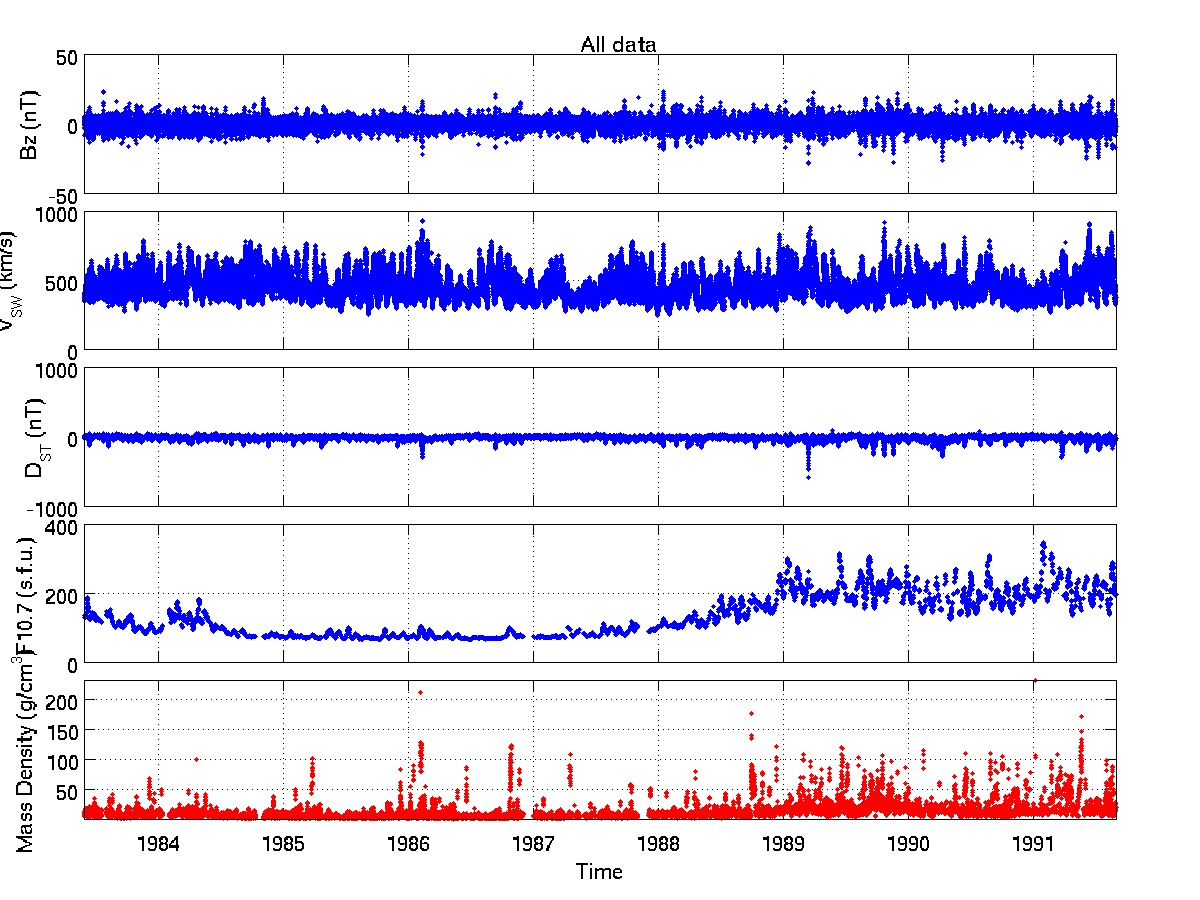
\includegraphics[scale=0.35]{paperfigures/alldata.png}
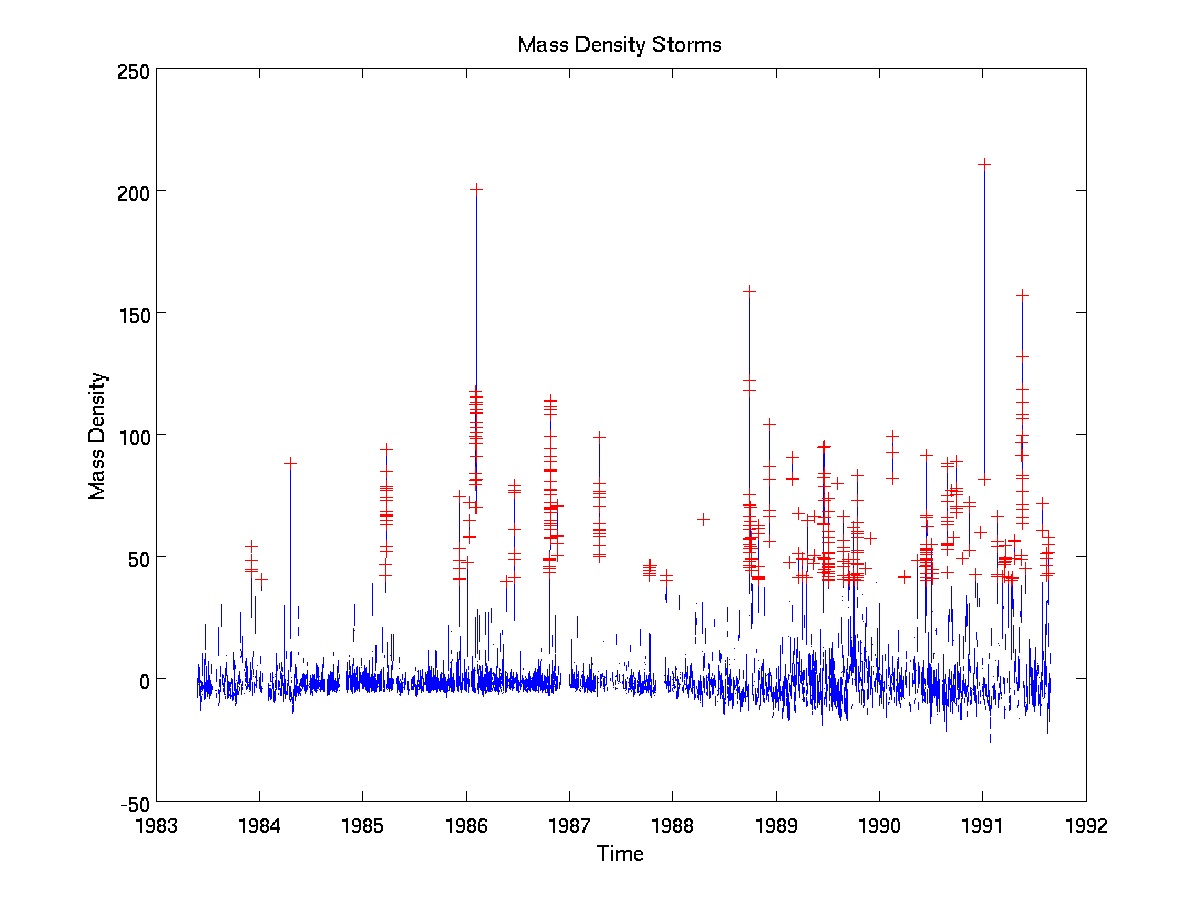
\includegraphics[scale=0.35]{paperfigures/massdensitystorms.png}
\caption{All used data (left) and selected storm times highlighted (right)}
\label{DSTstorm}
\end{figure}

This figure shows a definite spike in the $Z$ component of the magnetic field, as well as the defined drop in $DST$, but no obvious change in mass density as \citep{Takahashi} loosely suggests. 

\subsection{Mass Density Storm}
Figure \ref{MassStorm} shows this same algorithm, but looking for a rise in mass density over a value of 40$g/cm^3$. This results in 130 storms with a mean duration of 32 hours and a median duration of 17 hours, marked in red on the left figure.

\begin{figure}[htp!]
\centering
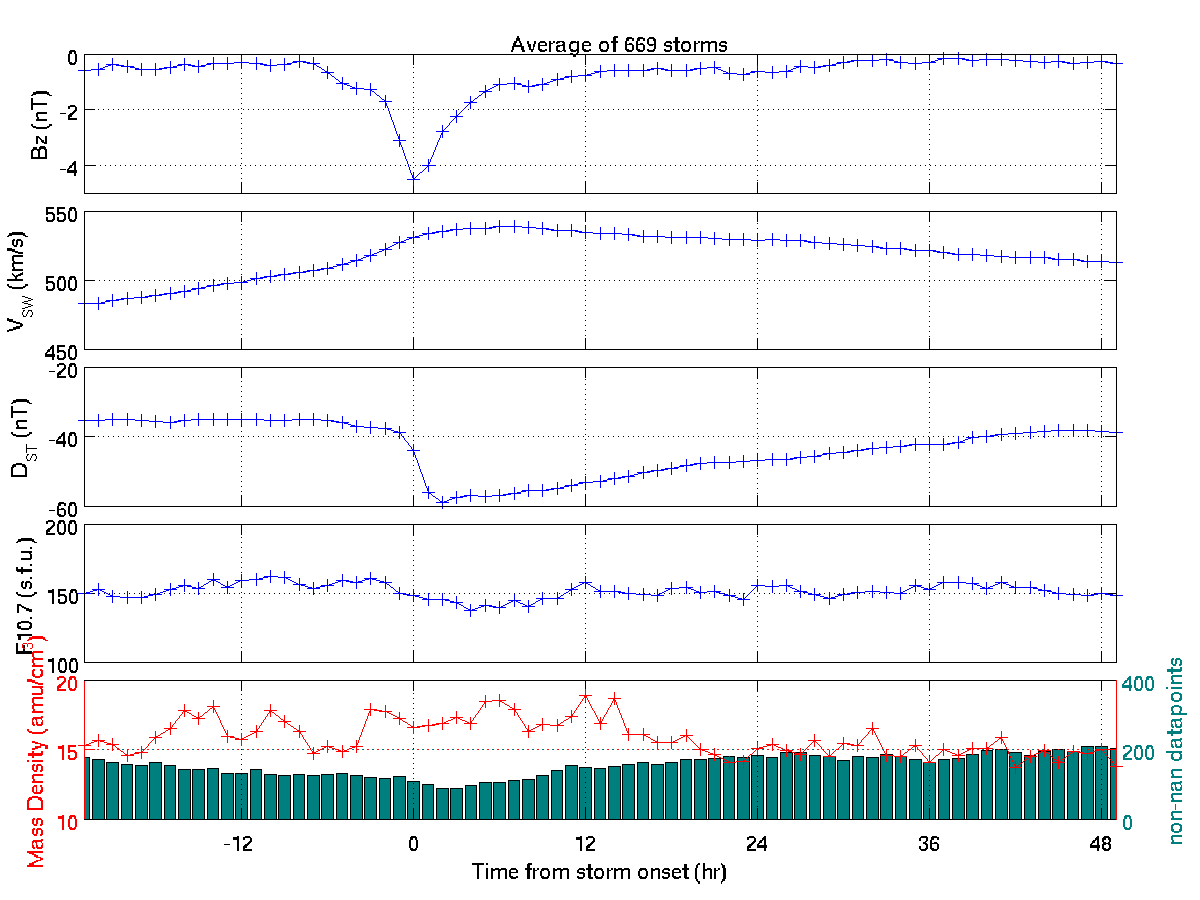
\includegraphics[scale=0.35]{paperfigures/stormavs-dst.png}
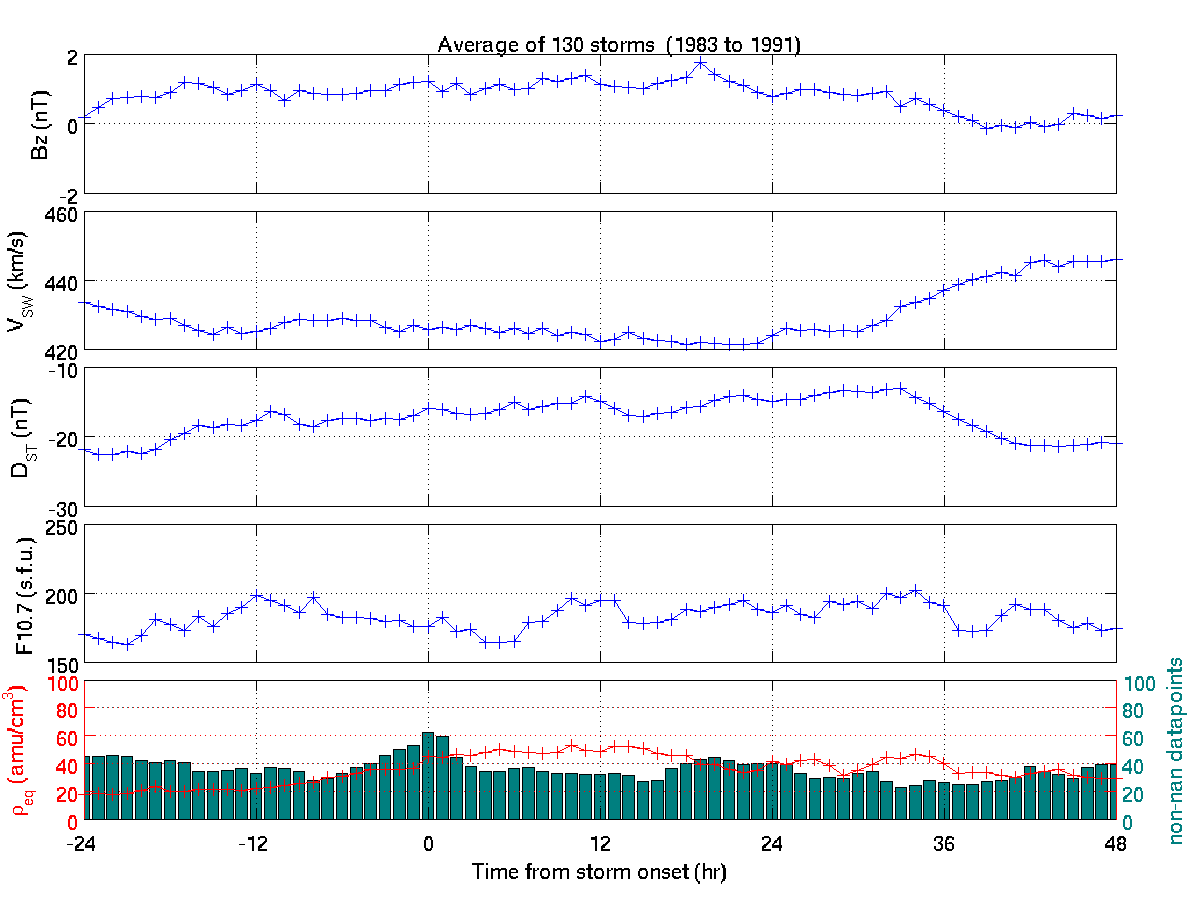
\includegraphics[scale=0.35]{paperfigures/stormavs-mass.png}
\caption{$D_{ST}<-40nT$ onset, Mass Density $>40 g/cm^3$}
\label{MassStorm}
\end{figure}

This shows that when using all data for mass density derived storms, almost no significant changes can be seen around storm onset.

\section{More specific storms}
It's hypothesized that progressively picking more specific storm criteria will allow for the possibility of more significant results, at the expense of more bias in the selection process and potentially less overall usefulness of the results. That said, the predictability of extreme storms is of definite interest, so an attempt has been made to find some reproducible method of prediction. Looking at storms that last longer than 12 hours and storms with an onset threshhold greater than $70g/cm^3$ results in the left and right sides of Figure \ref{Mspec} respectively.

\begin{figure}[htp!]
\centering
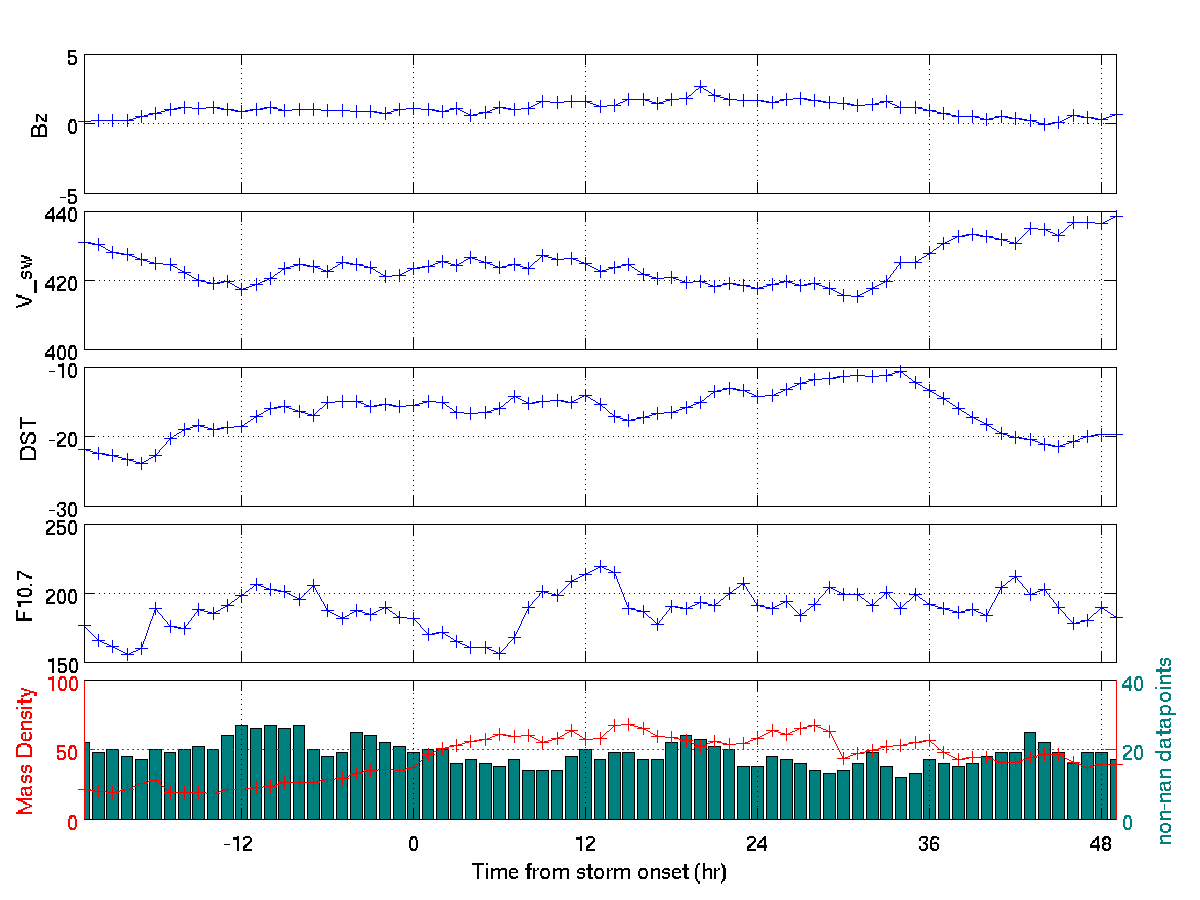
\includegraphics[scale=0.35]{paperfigures/stormavs-md12.png}
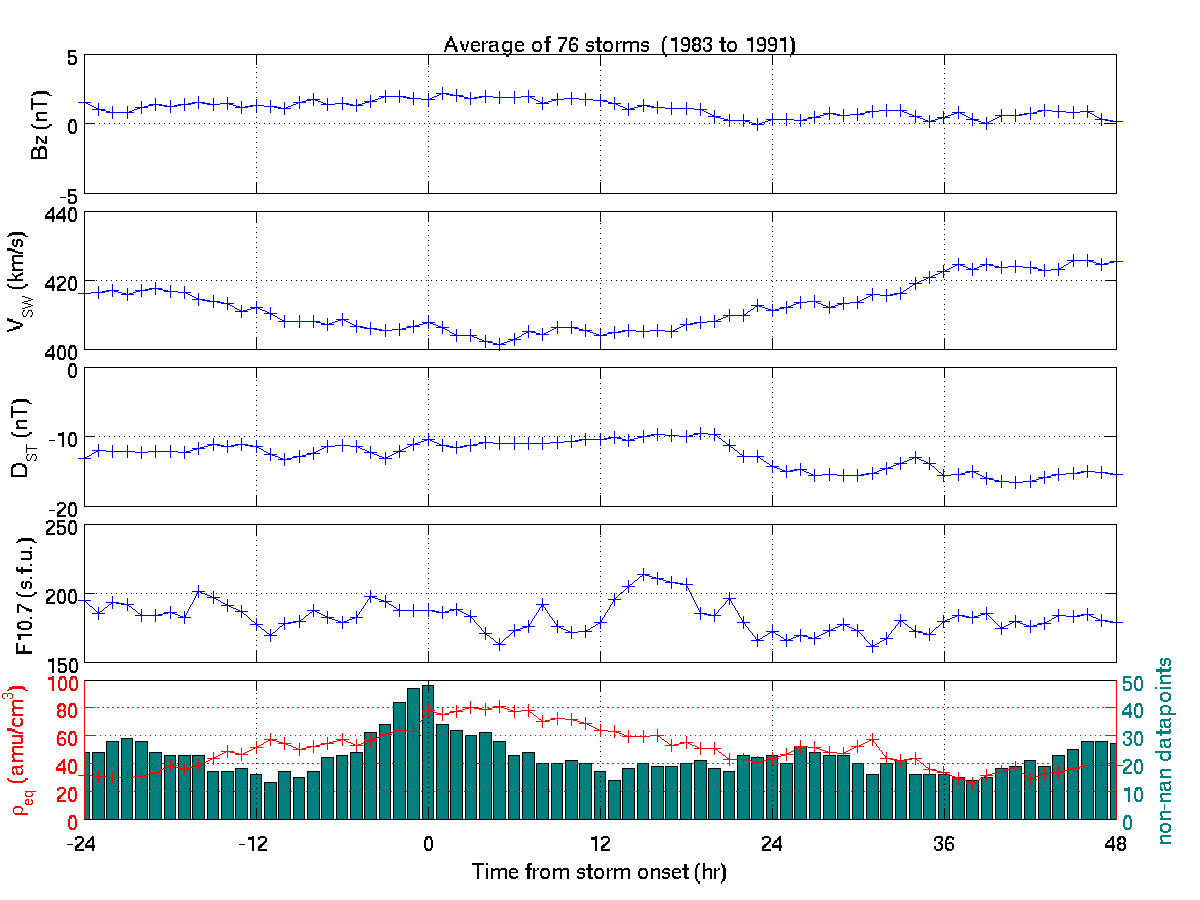
\includegraphics[scale=0.35]{paperfigures/stormavs-m70.png}
\caption{Specific Mass Density Storms}
\label{Mspec}
\end{figure}

Neither of these seem to indicate anything too significant, so looking at $D_{ST}$ storms instead to look for something that causes a significant change in Mass Density results in Figure \ref{Dspec}. This shows that by either looking only at $D_{ST}$ storms that last longer than an hour (left) or at storms where the onset condition is $D_{ST}<-80nT$, a spike in mass density is seen, but also a definite lack of data availability. 

\begin{figure}[htp!]
\centering
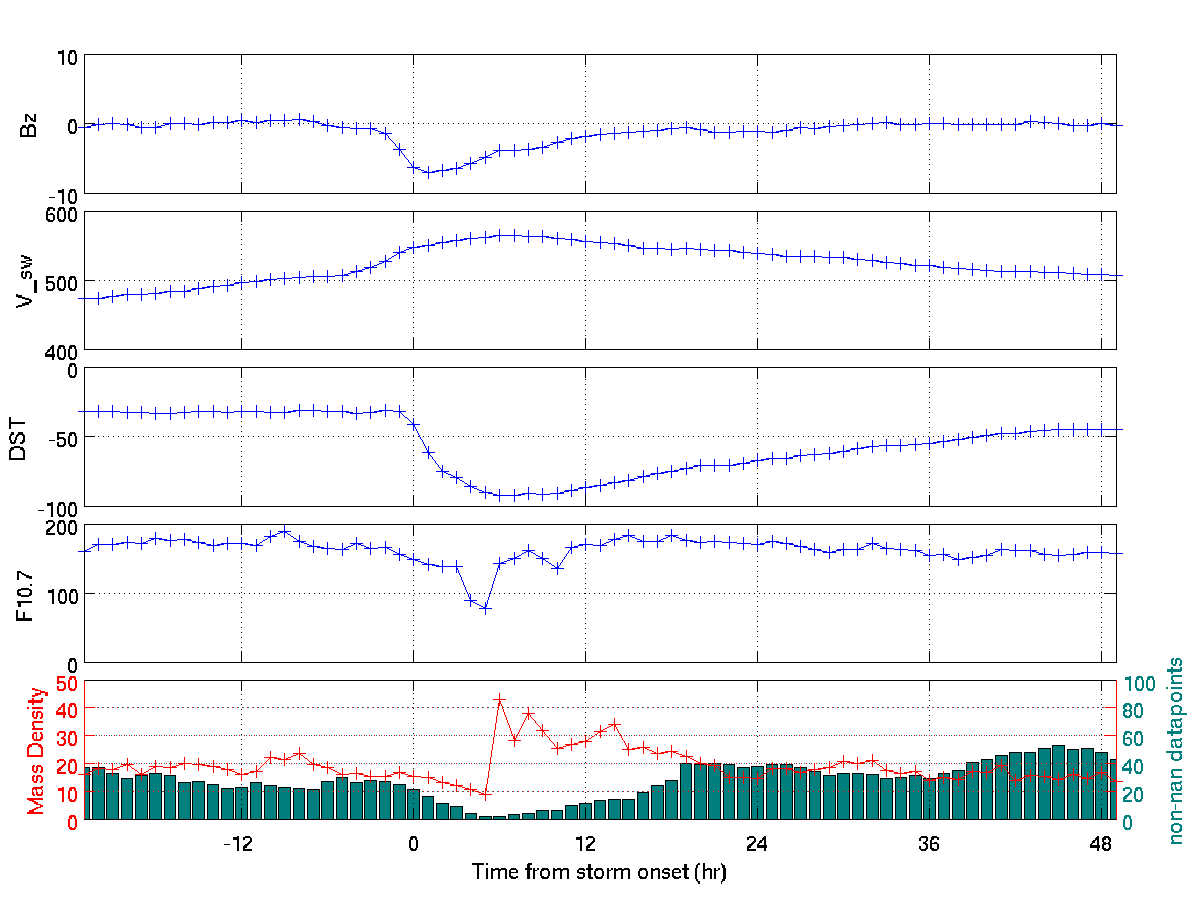
\includegraphics[scale=0.35]{paperfigures/stormavs-dd12.png}
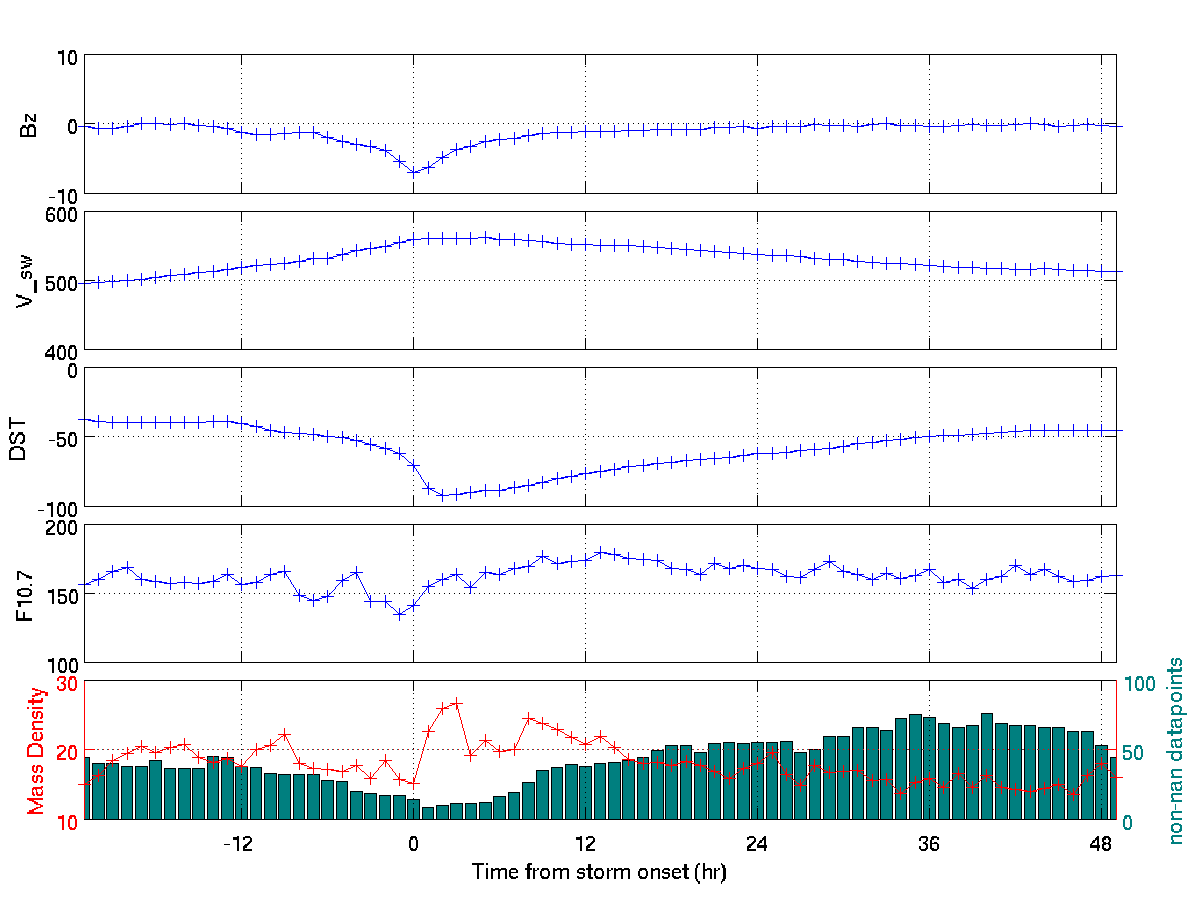
\includegraphics[scale=0.35]{paperfigures/stormavs-d80.png}
\caption{$D_{ST}$ Storms $>$ 12 hours, $D_{ST}<-80nT$}
\label{Dspec}
\end{figure}

\bibliographystyle{vplainnat}

\bibliography{reportbib}

\end{document}